\documentclass[11pt]{scrartcl}
\usepackage{geometry}                % See geometry.pdf to learn the layout options. There are lots.
\geometry{letterpaper}                   % ... or a4paper or a5paper or ... 
%\geometry{landscape}                % Activate for for rotated page geometry
%\usepackage[parfill]{parskip}    % Activate to begin paragraphs with an empty line rather than an indent
\usepackage{graphicx}
\usepackage{amssymb}
\usepackage{epstopdf}
\DeclareGraphicsRule{.tif}{png}{.png}{`convert #1 `dirname #1`/`basename #1 .tif`.png}

\usepackage{amsmath}

\title{Hierarchical Latent Space Models}
%\author{}
%\date{}                                           % Activate to display a given date or no date

\begin{document}
\maketitle
%\section{}
%\subsection{}

% Social network analysis % LOL -- and that's where I stopped
\begin{abstract}
NOTE: Discussions with an expert in matching methods led us to conclude that our project was somewhat ill-posed. We apologize for the change in directions, but believe that this project has a far greater potential for both interesting and valuable results, while also incorporating the material from the class in an important way.
\end{abstract}

\section{Motivation}
\subsection{Multigraph Data}
Social network analysis (SNA) is a very strange field, in a number of ways. it is inherently interdisciplinary, even its name indicating that it emphasizes both sophisticated statistical machinery, and also much more qualitative elements. While this is an exciting intersection, spanning both of these such disparate approaches is exceptionally difficult. As a result many important problems in SNA are under-studied, simply because of the small number of people who think about the problems it considers, in their full depth.

One of these problems is that of modeling multigraphs. Multigraphs, also called multiview networks, can be thought of as either a single graph with multiple edge types, or as multiple networks over the same set of nodes. Data of this kind is not uncommon, at either large or small scales. Twitter has Following relationships, as well as Retweets, and Likes, each of which can be thought of as simply one layer within the full relationship between two nodes. In small scales, surveys for networks very rarely ask about a single type of relationship, and many of the most famous network data sets have multiple relationships (such as Trust, Friendship, and Respect, in Samson's monk data). Despite the existence of data of this form for decades, the strange nature and inherent difficulty of this data has led to an extremely small number of ways to model it.


\subsection{Visualization and Comparability}
In designing a model however, the complexity of the data requires a perspective on what aspect of the network is most important. The model considered here was inspired initially by a very practical problem. A particular data set had five layers, and the goal was to compare visualizations of the five separate layers, to gain an intuition for similarities in the networks (visualization has long been a cornerstone of SNA, and graph layout algorithms is a substantial field unto itself). However, even if it has the same set of nodes, a graph with different sets of edges may be laid out completely differently -- incomparably -- from a graph with a different set of edges. The other approach, to immediately solve this problem of incomparable node placement, is to fix all of the positions a priori. However it has also long been known that doing so is the least informative visualization possible, as the very point of layout algorithms is to drive placement as a function of connectivity. This inspired the thought that perhaps a model could trade off these two extremes -- allowing just enough flexibility that the layout of a single layer could be both informative, and also compared meaningfully with the other layers in a graph. Such a model might take the following form.

\section{A Model}
\subsection{Latent Space Models}
First, after many years of development, network models of organization-scale systems have crystallized around a small number of well-developed paradigms. The most recent of these, but also now one of the most promising, is the family of Latent Space Models (LSMs). These assign a latent, k-dimensional variable to each node, and then attempt to place these variables such that nodes that share edges have their variables close together, and vice versa. 

\subsection{Previous Work}
Latent Space Models have been used to model multigraphs, with success, but also shortcomings.A recent paper proceeds by assigning each node k different latent variables (one for each network layer), and furthermore allowing correlations between the layers. This allows an edge to be explained either by two nodes in a particular layer being closer, or by two nodes in a correlated layer being close. While intuitively appealing, the designers of these models themselves describe the result as too flexible which is also not hard to believe. Furthermore, for the problem of comparable graph visualizations, because of this flexibility, these models would not solve the comparability problem described above.

\subsection{The Benefits of a Hierarchical Approach}
Another way forward, that does solve this problem, is to use a hierarchical model.

This model would have two distinct types of latent variables. It would start with a ``base''  latent position for each node. It would then give each node a set of $k$ latent variables that corresponded to the node's positions in the $k$ layers of the multigraph, but these positions would be constrained by the hierarchical ``base'' variable, and expressed as a perturbation away from its location. This approach would have multiple benefits.

\subsubsection{An Appropriate and Tunable Flexibility}
First, as mentioned, this model would not suffer the identifiability problems of the previous work, where a single edge could be the product of several completely distinct processes. Especially given that there are very few modern methods for modeling multigraphs, this is considered to be a non-trivial contribution to the SNA toolkit.

\subsubsection{The Solution to a Complex Visualization Problem}
Second, and again as mentioned above, this model could serve not only as a model, but also as a layout procedure. By choosing the latent variables all to be in two dimensions (which is also not necessary for the model to work -- it would retain the expressiveness of using higher dimensional latent spaces), the positions can be directly visualized, and compared. This is considered to be a particular strength of the approach.

\subsubsection{Dimensionality Reduction}
Last, but also substantially, the model very naturally admits a valuable process for dimensionality reduction. The ``tunability'' of the model stems from the ability to give different variances to the priors of the latent ``perturbations'' -- the distance that layer-specific latent positions can move away from the ``base'' position. However by using a sharp prior, and layer-specific variances, it is easy to regularize the layers so that if one is essentially a duplicate of another, the latent positions don't move at all. In other words, a sharp prior can lead to a redundant layer of the multigraph being omitted -- a crucial ability, when the complex new model is motivated entirely by there being an unwieldy number of layers to begin with.


% Using different priors on the widths of these perturbations would go from layers that were identical (and thus comparable) to models that were essentially independent. Consequently, the model could be explicitly tuned to find an optimal balance between expressiveness and flexibility. 

% In addition, the use of a parameter-wise, or group LASSO penalty on the model, could either eliminate meaningless small perturbations on single nodes, or on entire layers of the graph. In other words, a group LASSO could be used as a multigraph dimensionality reduction technique, reducing a five layer network to only two ``meaningful'' layers -- an important problem without an obvious solution otherwise, given the tensor structure of the data.

\section{Fitting the Proposed Model}
%NO idea, fuck. K then. So -- it's important to actually think about now then, though. So ... also tell them soon. 
\subsection{The Optimization Problem}
%The optimization problem has a slightly different from from any we have studied so far -- it is a group-lasso, but with equality constraints.
The optimization problem can be written as

\begin{align*}
\min_{z,b} &\sum_{ij} r_{ij}^2 + \lambda \sum_k \|\epsilon_k\|_2\\
%& \:\:\: \text{ s.t. } z_{ik} = b_i + \epsilon_{ik}
\end{align*}

where $r_{ij} = e_{ijk} - \sigma(\alpha_k - d_{ijk})$ are the residuals of the edge predictions, and $d_{ijk} = \|b_i + \epsilon_{ik} - b_j - \epsilon_{jk}\|^2_2$ are the distances between nodes $i$ and $j$ in graph layer $k$. The vectors $\epsilon_k$ encode the layer-wise deviations from the base positions, so that a group penalty on $\epsilon_k$ essentially forces the layer $k$ to be expressed only in terms of the base positions $b$. This is the penalty that produces layer-wise dimensionality reduction.

\subsection{Stan}
The proposed model can be easily expressed in the Bayesian modeling language Stan, the modern replacement to the widely-used language BUGS. However, testing the model requires a substantial amount of both work, and time, given how slow the models are to fit. In addition, a theoretical understanding of the model is not very developed at this point, and this development is expected to lead to many insights that would greatly improve the speed of fitting at the very least, as well as potentially many other issues. Stan is thus the starting point and valuable proof of concept, but the optimization techniques learned in the class are expected to take this proof of concept and turn it into a far more practical and reliable analytic tool. 

In particular, the multiple analyses we have performed using the LASSO are expected to be extremely valuable in understanding how to properly fit this penalized model.

\subsection{Current Progress}
Two important steps have been made. The first is that a simple version of the original LSM was coded to make sure that it would work properly in the modeling language being used. The results were as hoped. The second step, given the success of the first, was to implement this novel HLSM in the same modeling language. This has been accomplished, and now we can begin to make substantial progress into improving and analyzing the model.

%\section{The Current State of the Model}

\begin{figure}
	\centering
	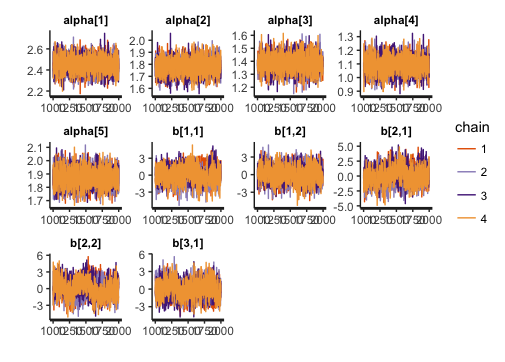
\includegraphics[width=4in]{hlsm_traceplot}
	\caption{Sampling Chains for the HLSM}
	\label{fig:chains}
\end{figure}

\section{Next Steps}
\subsection{Issues to Resolve}
While the model runs, which is considered to be a substantial success on its own, given the complexity, there are visible issues with fitting some of the parameters -- the latent positions, in particular. The initial trial was to fit the novel data set that motivated the models development. A trace plot of the sampling chains can be see in Figure \ref{fig:chains}, which demonstrates what is believed to be the major issue. While the intercept parameters are estimated without issue, the chains for the latent positions are not mixing fully, and the outcome positions are all very close to zero. There are multiple ways to resolve this, which include increasing the length of the chain, and starting from a better initialization, but a deeper and longer-term solution is to understand the theory behind the model better, and intentionally exploit its structure to either reparameterize the model so that sampler is more effective, or to fit it in an entirely different way. 

\subsection{Test Cases}
While the model did not initially perform as hoped for natural data, that is also not the best place to start. We are currently designing test cases for the model that would allow us to better understand, and debug, its behavior. Given the complexity of the model, the data it takes, and the large number of qualities the model possesses, this is not a simple task. The simulations that test model fit are quite different from the simulations used to assess data reduction, which are again different from the simulations used to assess the quality of the visualizations. A thorough suite of these will comprise the next steps in the project. These tests will show us where to focus our efforts, and also may themselves give us valuable insights into the workings and theory of the model.





\section{Bibliography}

Hoff, Peter D., Adrian E. Raftery, and Mark S. Handcock. \textit{Latent space approaches to social network analysis.} Journal of the american Statistical association 97.460 (2002): 1090-1098.\\

Salter-Townshend, Michael, and Tyler H. McCormick. \textit{Latent space models for multiview network data}. Technical Report 622, Department of Statistics, University of Washington, 2013.\\

Salter-Townshend. M, \textit{Personal communication}, 2017\\

Bob Carpenter, Andrew Gelman, Matthew D. Hoffman, Daniel Lee, Ben Goodrich, Michael Betancourt, Marcus Brubaker, Jiqiang Guo, Peter Li, and Allen Riddell. \textit{Stan: A probabilistic programming language}. Journal of Statistical Software 76(1). DOI 10.18637/jss.v076.i01, 2017\\

Loewi, A., \textit{Parent-Teacher Relationships and Student Outcomes}, 2017

% \section{Next Steps}



%-- and furthermore, rarely ask binary questions (are you friends, yes or no) about those relationships.


\end{document} 